\documentclass{beamer}
\usepackage[utf8]{inputenc}

\usetheme{Madrid}
\usecolortheme{default}
\usepackage{amsmath,amssymb,amsfonts,amsthm}
\usepackage{txfonts}
\usepackage{tkz-euclide}
\usepackage{listings}
\usepackage{adjustbox}
\usepackage{array}
\usepackage{tabularx}
\usepackage{gvv}
\usepackage{lmodern}
\usepackage{circuitikz}
\usepackage{tikz}\documentclass{beamer}
\usepackage[utf8]{inputenc}

\usetheme{Madrid}
\usecolortheme{default}
\usepackage{amsmath,amssymb,amsfonts,amsthm}
\usepackage{txfonts}
\usepackage{tkz-euclide}
\usepackage{listings}
\usepackage{adjustbox}
\usepackage{array}
\usepackage{tabularx}
\usepackage{gvv}
\usepackage{lmodern}
\usepackage{circuitikz}
\usepackage{tikz}
\usepackage{graphicx}

\setbeamertemplate{page number in head/foot}[totalframenumber]

\usepackage{tcolorbox}
\tcbuselibrary{minted,breakable,xparse,skins}



\definecolor{bg}{gray}{0.95}
\DeclareTCBListing{mintedbox}{O{}m!O{}}{%
  breakable=true,
  listing engine=minted,
  listing only,
  minted language=#2,
  minted style=default,
  minted options={%
    linenos,
    gobble=0,
    breaklines=true,
    breakafter=,,
    fontsize=\small,
    numbersep=8pt,
    #1},
  boxsep=0pt,
  left skip=0pt,
  right skip=0pt,
  left=25pt,
  right=0pt,
  top=3pt,
  bottom=3pt,
  arc=5pt,
  leftrule=0pt,
  rightrule=0pt,
  bottomrule=2pt,

  colback=bg,
  colframe=orange!70,
  enhanced,
  overlay={%
    \begin{tcbclipinterior}
    \fill[orange!20!white] (frame.south west) rectangle ([xshift=20pt]frame.north west);
    \end{tcbclipinterior}},
  #3,
}
\lstset{
    language=C,
    basicstyle=\ttfamily\small,
    keywordstyle=\color{blue},
    stringstyle=\color{orange},
    commentstyle=\color{green!60!black},
    numbers=left,
    numberstyle=\tiny\color{gray},
    breaklines=true,
    showstringspaces=false,
}
%------------------------------------------------------------
%This block of code defines the information to appear in the
%Title page
\title %optional
{1.5.2}
\date{August  2025}
%\subtitle{A short story}

\author % (optional)
{Bhoomika L - EE25BTECH11014}

\begin{document}


\frame{\titlepage}
\begin{frame}{Question}
 Find the ratio in which the \textit{Y} axis divides the line segment joining the points $\brak{6,-4}$ and $\brak{-2,-7}$. Also find the point of intersection.
 \end{frame}

\begin{frame}{Theoretical Solution}
Given the points,
\begin{align}
    \vec{A}=\begin{myvec}{6\\-4}\end{myvec}
    \vec{B}=\begin{myvec}{-2\\-7}\end{myvec}
\end{align}

Let the vector $\vec{P}$ be 
\begin{align}
    \vec{P}=\begin{myvec}{0\\y}\end{myvec} \;, 
\end{align}
The points \textbf{A},\textbf{P},\textbf{B} are collinear.
\end{frame}

\begin{frame}{Formulae}
The points to be collinear,
\begin{align}
	\label{eq:line-rank-2}
	\rank{\myvec{\vec{P}-\vec{A}& \vec{B}-\vec{A}}} = 1\\
\end{align}
\end{frame}

\begin{frame}{Theoretical Solution}
\begin{align}
  \vec{P}-\vec{A} = \myvec{-6\\y+4}\\
         \vec{B}-\vec{A} = \myvec{-8\\-3}\\
        \myvec{\vec{P}-\vec{A}& \vec{B}-\vec{A}} = \myvec{-6 & -8\\ y+4&-3 }
 \end{align}
 
\begin{center}
 Conversion to Row Echelon form,
$R_2 \rightarrow R_2 + \frac{y+4}{6}R_1 :$ 
\myvec{ -6 & -8\\0 & -3+ \frac{y+4}{6}(-8)}\implies
\myvec {-6 & -8\\0 & \frac{-4y-25}{3}}\\
\end{center}
 \begin{align}
 \frac{-4y-25}{3}=0\implies y=-\frac{25}{4}
 \end{align}
  \begin{center}
      $\therefore \vec{P}=\begin{myvec}{0\\-\frac{25}{4}}\end{myvec}$
 \end{center}
 \end{frame}

 \begin{frame}{Formulae}
\textbf{Section formula for a vector $\vec{P}$ which divides the line formed by vectors $\vec{A}$ and $\vec{B}$ in the ratio k:1 is given by}
\begin{align}
    \vec{P}=\frac{k\vec{B}+\vec{A}}{k+1}
\end{align}
\begin{align}
			k\brak{\vec{P}-\vec{B}}&= \vec{A}-\vec{P}
\end{align}
\begin{align}\implies k &=
			\frac{\brak{\vec{A}-\vec{P}}^{\top}\brak{\vec{P}-\vec{B}}}{\norm{\vec{P}-\vec{B}}^2}
			\label{eq:section_formula-k}
\end{align}
\end{frame}

\begin{frame}{Theoretical Solution}
\begin{align}
\brak{\vec{A}-\vec{P}}^{\top}\brak{\vec{P}-\vec{B}} =\myvec{6 & \frac{9}{4}}\myvec{2\\ \frac{3}{4}
}=\frac{219}{16}\\
{\norm{\vec{P}-\vec{B}}^2} = \brak{\sqrt{2^2 + {\brak{\frac{3}{4}}}^2}}^2 = \frac{73}{16}\\
k=\frac{\frac{219}{16}}{\frac{73}{16}}
\end{align}
 \begin{align}
\implies k &= 3
\end{align}
 Therefore the ratio in which point \textbf{P} divides the line segment joining \textbf{A} and \textbf{B} is 3:1
\end{frame}

\begin{frame}[fragile]
    \frametitle{C Code }

    \begin{lstlisting}
#include <stdio.h>

// Section formula: returns y-coordinate when x=0
float sec_form(int x1, int y1, int x2, int y2, int *m, int *n, float *px, float *py) {
    // Compute ratio
    *m = x1;
    *n = -x2;

    // Point of intersection (x=0)
    *px = 0.0;
    *py = (*m * y2 + *n * y1) / (float)(*m + *n);

    return *py;
}

\end{lstlisting}
\end{frame}

\begin{frame}[fragile]
    \frametitle{Python Code}
    \begin{lstlisting}
import numpy as np
import matplotlib.pyplot as plt

# --- Define points ---
A = np.array([6.0, -4.0])
B = np.array([-2.0, -7.0])

# --- Function to generate a line segment between two points ---
def generate_line_segment(point1, point2, num_points=50):
    line_segment = np.zeros((2, num_points))
    lambda_vals = np.linspace(0, 1, num_points)
    for i in range(num_points):
        temp = point1 + lambda_vals[i] * (point2 - point1)
        line_segment[:, i] = temp.T
    return line_segment

  \end{lstlisting}
\end{frame}

\begin{frame}[fragile]
    \frametitle{Python Code}
    \begin{lstlisting}
# --- Generate line AB ---
x_AB = generate_line_segment(A, B)

# --- Plot line AB ---
plt.plot(x_AB[0, :], x_AB[1, :], label='$AB$')

# --- Plot points A and B ---
all_points = np.vstack((A, B)).T
plt.scatter(all_points[0, :], all_points[1, :], color='red')

\end{lstlisting}
\end{frame}

\begin{frame}[fragile]
    \frametitle{Python Code}
    \begin{lstlisting}
# --- Add labels ---
point_labels = [f'A {tuple(A)}', f'B {tuple(B)}']
offsets = [(10, 5), (-30, -10)]
for i, txt in enumerate(point_labels):
    plt.annotate(txt,
                 (all_points[0, i], all_points[1, i]),
                 textcoords="offset points",
                 xytext=offsets[i],
                 ha='center')
    \end{lstlisting}
    \end{frame}

\begin{frame}[fragile]
    \frametitle{Python Code}
    \begin{lstlisting}

# --- Plot settings ---
plt.xlabel('$x$')
plt.ylabel('$y$')
plt.title('Line segment AB')
plt.legend(loc='best')
plt.grid(True)
plt.axis('equal')

# --- Save and show plot ---
plt.savefig('../Figs/graph.png')
plt.show()
    \end{lstlisting}
    \end{frame}



\begin{frame}{Plot}
    \centering
    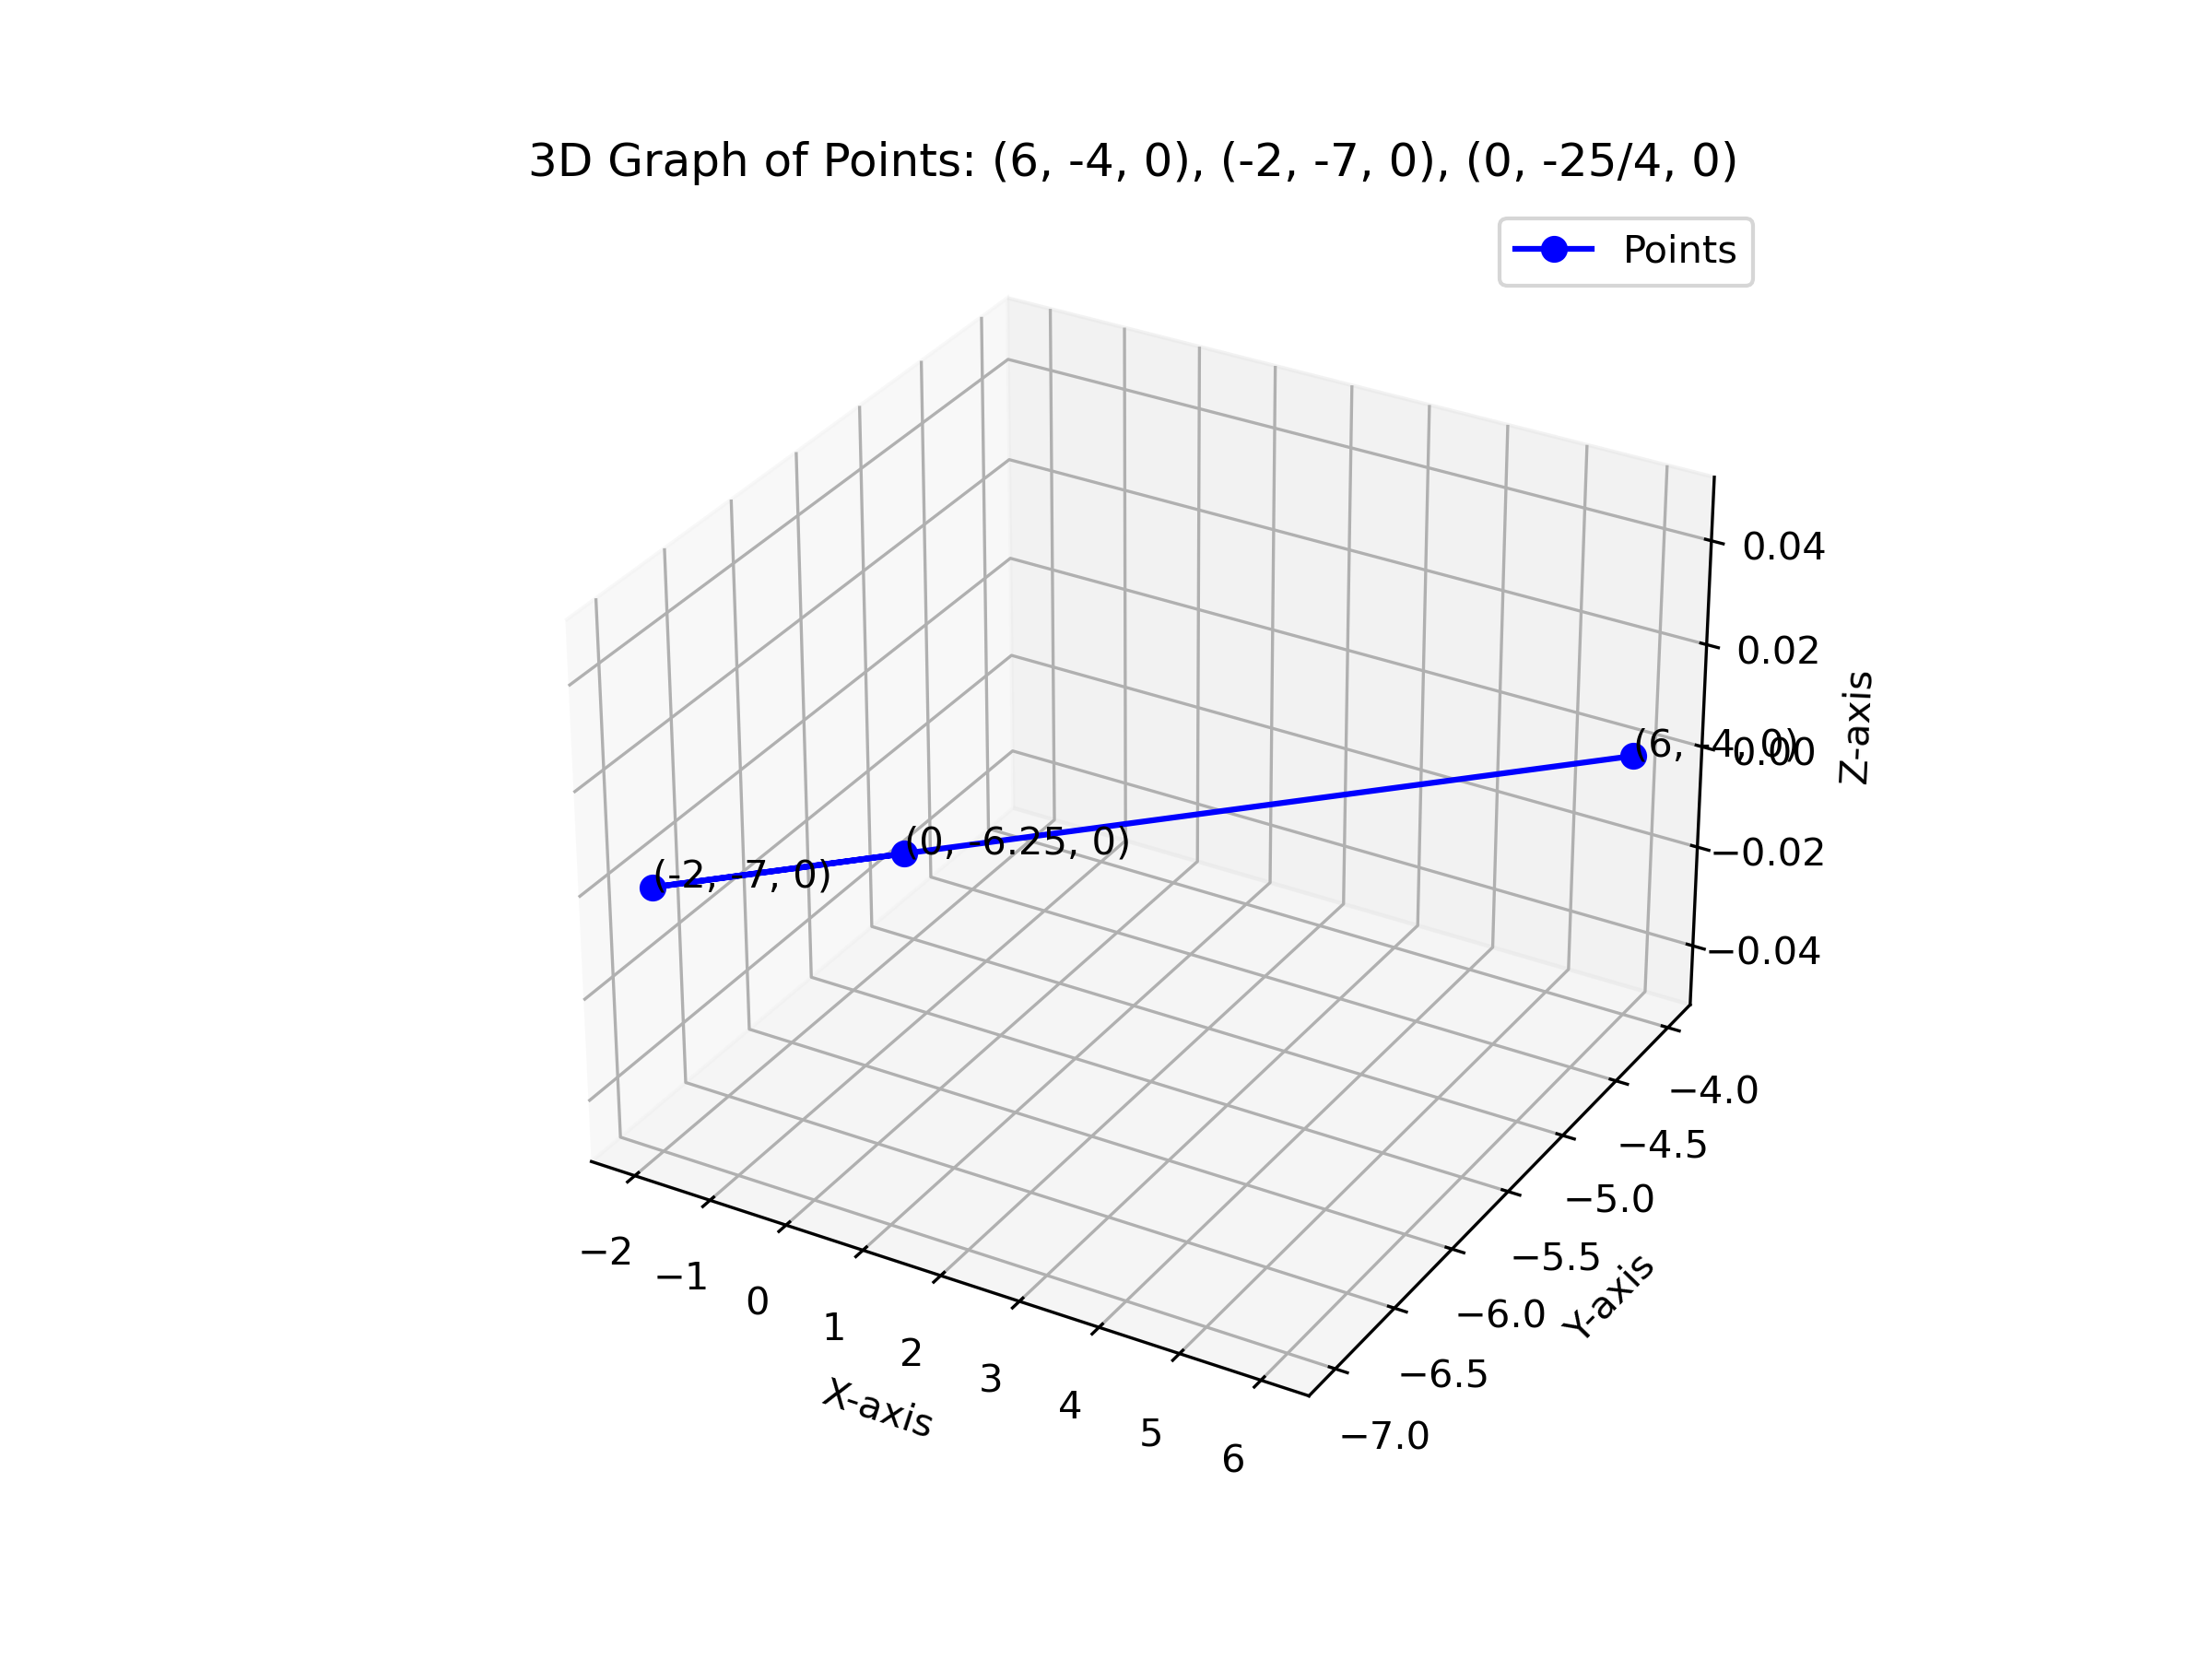
\includegraphics[width=\columnwidth, height=0.8\textheight, keepaspectratio]{../Figs/graph3d.png}     
\end{frame}

\end{document}

